\documentclass{article}
\usepackage{graphicx}
\usepackage{subcaption}
\usepackage{geometry}
\usepackage{tikz}
\usepackage{amsmath}
\usepackage{cleveref}
\usepackage{float}
\usepackage[useregional]{datetime2}
\def\checkmark{\tikz\fill[scale=0.4](0,.35) -- (.25,0) -- (1,.7) -- (.25,.15) -- cycle;}
\usepackage[font=small,skip=0pt]{caption}
\geometry{legalpaper, margin=1in}
\title{STAT 8003 Homework 1}
\author{Zhijia Chen}
\date{\today}

\begin{document}

\begin{titlepage}
    \maketitle
\end{titlepage}



Stock performance forecast is always an intriguing topic. Many indexes has been proposed as indicator for the market performance, within which the S\&P 500 index is arguably the most widely recognized. The S\&P 500 index is a composite index of 500 largest U.S. stocks and it generally shows the overall performance of the whole stock market.Thus S\&P 500 prediction is of great interests in the field of market forecast. While predicting S\&P 500 based on relevant variables might produce a stable model that is more tolerant of market disturbance, it requires a deep insight of the market and tremendous efforts in sorting out accurate relationships between the index and it's dependent variables, predicting the future of the S\&P 500 solely based on it's past, however, is a much simpler method. In this study, we show that ARMA model, or Autoregressive Moving Average model, is able to fit the S\&P 500 annual returns very well, and can also produce a reliable prediction of changes in the near future. We used the returns after 1950 to fit the ARMA model and use the last 12 months (Jan, 2017 ~ Dec, 2017) to test the forecast. The AIC and BIC for the fitted data are pretty low, with the former being -2.664e+03 and and the later being -2.580e+03, while they are much higher for the forecasted data but yet are still acceptable, as AIC being ? and BIC ? respectively. But we do notice that the changes in the fitted data usually lag behind the actual data, and the error of the forecast data increases as the forecast span increases. The ARMA model might not able to produce an accurate prediction, especially when there are dramatic changes, but when only the short time trend is of interest, it's much more efficient compared to those modeling methods such as linear regression that requires finding the dependent variables of the target variable and the corresponding relationships.

In this study, our goal is to forecast the annual returns of the S\&P 500 index after 1950. We use the ARMA model to fit the data and try to do a 1-year-span forecast. An ARMA model, or Autoregressive Moving Average model, is used to describe weakly stationary stochastic time series in terms of two polynomials. The first of these polynomials is for autoregression, the second for the moving average[https://www.statisticshowto.datasciencecentral.com/arma-model/]. The model is usually referred as the $$ARMA(p,q)$$ Model.



See figure ~\ref{fig:sp500}.

\begin{figure}[H]
    \centering
        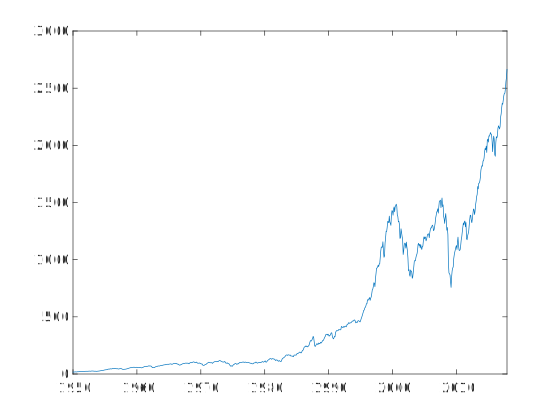
\includegraphics[width=0.8\textwidth]{sp500}
    \caption{S\&P 500 Index After 1950}
    \label{fig:sp500}
\end{figure}


\end{document}

